% LXTUL: measured results (README figure, below the mechanism drawing). Drawn 2026-10-07.
% Split out of the old tul_mechanism.tex MEASURED box on Wolfe's feedback (2026-10-07).
%
% Every number, copied from the README results table and its filings (no re-rounding):
%   plain looped model (no pointer): CE@6 4.0806, gap 0, seq_rep_4 0.215
%     (lab/experiments/mixed/2026-10-06-lxtul-pointer.md results table, "reference: plain
%     ruler"; seq_rep_4: lab/experiments/failures/2026-10-07-lxtul-pointer-coverage.md, "plain").
%   LXTUL: CE@6 4.3529, gap +0.272, K1-K6 +0.0215 (seed 1), seq_rep_4 0.041
%     (.agents/notes/implemented/architecture/2026-10-04-lxtul-primary-candidate.md, 5k seed 1;
%     2026-10-06-lxtul-pointer.md reference row; seq_rep_4: coverage filing "LXTUL, no head").
%   LXTUL + pointer, 5k: CE@6 3.9280, gap -0.150 [-0.169, -0.132] (filing: -0.1497 [-0.1690,
%     -0.1320]; README rounds to 3 places), K1-K6 +0.0155, seq_rep_4 0.307
%     (2026-10-06-lxtul-pointer.md; seq_rep_4: coverage filing "pointer 5k").
%   + DITTO phase, 1000 steps: trainer val +0.071 vs its control phase (4.0254 vs 3.9548),
%     sweep K1-K6 +0.0294 on rows the phase re-trained, seq_rep_4 0.140 (control phase 0.291)
%     (lab/experiments/mixed/2026-10-07-lxtul-pointer-ditto.md).
%   real text seq_rep_4 0.020 (both generation filings).
% seq_rep_4 = 4-gram repetition of sampled text at temperature 0.7, top-k 40, 24 prompts.
% K1-K6 = CE at loop depth 1 minus CE at depth 6.
%
% Bar scales: CE gap 10 cm per nat (zero axis at x = 7.4); K1-K6 100 cm per nat (from
% x = 11.4); seq_rep_4 8 cm per unit (from x = 15.4). Bars are exact to the plotted value.
% Palette: Paul Tol (as morph_overview.tex); no meaning rides on hue (each column has one
% hue; the re-trained-rows reading is marked by a dashed outline and a dagger).
% Compile: pdflatex tul_results.tex
%          pdftoppm -png -r 220 -singlefile tul_results.pdf ../tul_results

\documentclass[border=16pt]{standalone}
\usepackage[T1]{fontenc}
\usepackage{amsmath,amssymb}
\usepackage{tikz}
\usetikzlibrary{arrows.meta, positioning, calc}

\definecolor{cbBlue}{HTML}{4477AA}
\definecolor{cbOrange}{HTML}{EE7733}
\definecolor{cbPurple}{HTML}{AA3377}
\definecolor{fBlue}{HTML}{DCEAF7}
\definecolor{fOrange}{HTML}{FDE8D0}
\definecolor{fPurple}{HTML}{EEDCEE}
\definecolor{fGray}{HTML}{EBEBEB}
\definecolor{bdr}{HTML}{555555}

\tikzset{
  row/.style={font=\large\sffamily, anchor=west, align=left},
  hd/.style={font=\large\sffamily\bfseries, anchor=south west, align=left},
  sh/.style={font=\small\sffamily, text=bdr, anchor=north west, align=left},
  val/.style={font=\sffamily, anchor=north west, align=left},
  barCE/.style={draw=cbBlue, thick, fill=fBlue},
  barK/.style={draw=cbPurple, thick, fill=fPurple},
  barR/.style={draw=cbOrange!85!black, thick, fill=fOrange},
}

% row centre y values
\def\yA{-1.6}
\def\yB{-3.0}
\def\yC{-4.4}
\def\yD{-5.8}
% bar half-height
\def\bh{0.22}
% CE zero axis, K1-K6 origin, repetition origin
\def\xCE{7.4}
\def\xK{11.4}
\def\xR{15.4}

\begin{document}
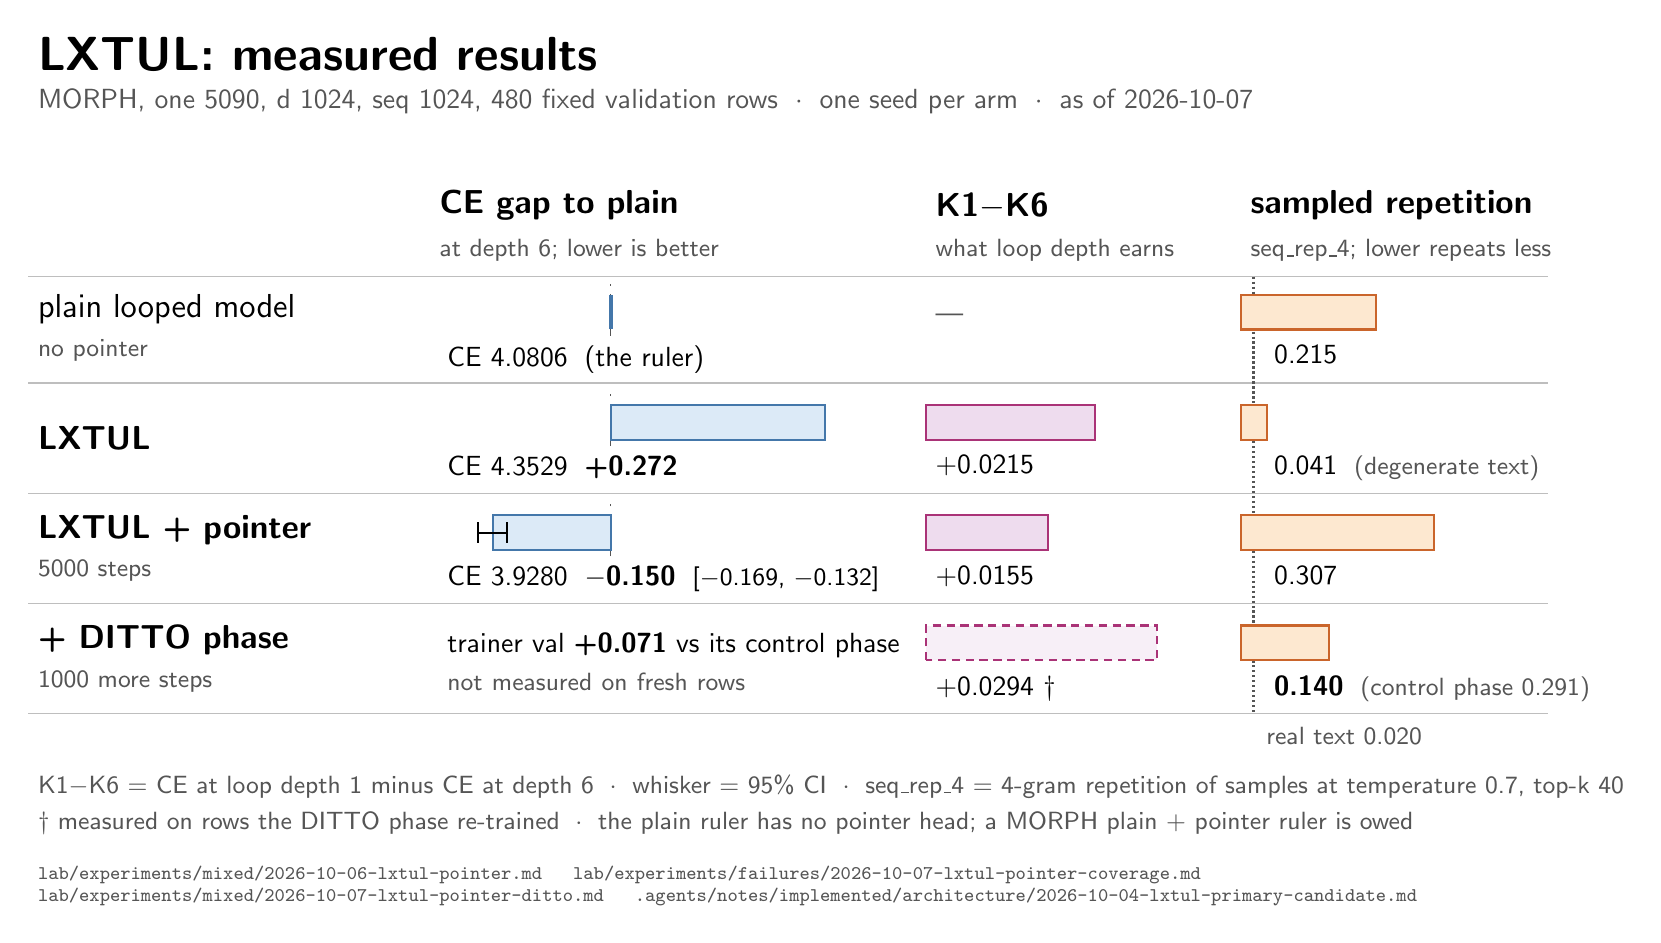
\begin{tikzpicture}

% ── title ────────────────────────────────────────────────────────────────────
\node[font=\LARGE\sffamily\bfseries, anchor=south west] (title) at (0, 1.55)
  {LXTUL: measured results};
\node[font=\sffamily, text=bdr, anchor=north west] at (title.south west)
  {MORPH, one 5090, d 1024, seq 1024, 480 fixed validation rows \;$\cdot$\; one seed per arm
  \;$\cdot$\; as of 2026-10-07};

% ── column headers ───────────────────────────────────────────────────────────
\node[hd] at (5.1, -0.35) {CE gap to plain};
\node[sh] at (5.1, -0.35) {at depth 6; lower is better};
\node[hd] at (\xK, -0.35) {K1$-$K6};
\node[sh] at (\xK, -0.35) {what loop depth earns};
\node[hd] at (\xR, -0.35) {sampled repetition};
\node[sh] at (\xR, -0.35) {seq\_rep\_4; lower repeats less};

% row separators
\foreach \y in {-0.95, -2.3, -3.7, -5.1, -6.5}
  \draw[fGray!70!bdr, thin] (0, \y) -- (19.3, \y);
% CE zero axis
\foreach \y in {\yA, \yB, \yC}
  \draw[bdr, dashed, thin] (\xCE, {\y+0.2-0.3}) -- (\xCE, {\y+0.2+0.36});
% real-text reference line in the repetition column (0.020 x 8 cm = 0.16 cm)
\draw[bdr, densely dotted, thick] ({\xR+0.16}, -0.95) -- ({\xR+0.16}, -6.5);
\node[font=\small\sffamily, text=bdr, anchor=north west] at ({\xR+0.2}, -6.55) {real text 0.020};

% ── row labels ───────────────────────────────────────────────────────────────
\node[row] at (0, \yA) {plain looped model\\{\small\color{bdr}no pointer}};
\node[row] at (0, \yB) {\textbf{LXTUL}};
\node[row] at (0, \yC) {\textbf{LXTUL + pointer}\\{\small\color{bdr}5000 steps}};
\node[row] at (0, \yD) {\textbf{+ DITTO phase}\\{\small\color{bdr}1000 more steps}};

% ── CE gap column (10 cm per nat) ────────────────────────────────────────────
% plain: the ruler, gap 0
\draw[cbBlue, very thick] (\xCE, {\yA+0.2-\bh}) -- (\xCE, {\yA+0.2+\bh});
\node[val] at ({\xCE-2.2}, {\yA-0.1}) {CE 4.0806 \;(the ruler)};
% LXTUL: +0.272 -> 2.72 cm
\draw[barCE] (\xCE, {\yB+0.2-\bh}) rectangle ({\xCE+2.72}, {\yB+0.2+\bh});
\node[val] at ({\xCE-2.2}, {\yB-0.1}) {CE 4.3529 \;\textbf{+0.272}};
% LXTUL + pointer: -0.150 -> -1.50 cm; 95% CI [-0.169, -0.132] -> [-1.69, -1.32]
\draw[barCE] ({\xCE-1.50}, {\yC+0.2-\bh}) rectangle (\xCE, {\yC+0.2+\bh});
\draw[black, thick] ({\xCE-1.69}, {\yC+0.2}) -- ({\xCE-1.32}, {\yC+0.2});
\draw[black, thick] ({\xCE-1.69}, {\yC+0.2-0.13}) -- ({\xCE-1.69}, {\yC+0.2+0.13});
\draw[black, thick] ({\xCE-1.32}, {\yC+0.2-0.13}) -- ({\xCE-1.32}, {\yC+0.2+0.13});
\node[val] at ({\xCE-2.2}, {\yC-0.1}) {CE 3.9280 \;\textbf{$-$0.150} \;{\small [$-$0.169, $-$0.132]}};
% DITTO: no fresh-row CE; trainer val vs its control phase
\node[val, text width=6.2cm] at ({\xCE-2.2}, {\yD+0.45})
  {trainer val \textbf{+0.071} vs its control phase\\[2pt]{\small\color{bdr}not measured on fresh rows}};

% ── K1-K6 column (100 cm per nat) ────────────────────────────────────────────
\node[val, text=bdr] at (\xK, {\yA+0.35}) {---};
\draw[barK] (\xK, {\yB+0.2-\bh}) rectangle ({\xK+2.15}, {\yB+0.2+\bh});
\node[val] at (\xK, {\yB-0.1}) {+0.0215};
\draw[barK] (\xK, {\yC+0.2-\bh}) rectangle ({\xK+1.55}, {\yC+0.2+\bh});
\node[val] at (\xK, {\yC-0.1}) {+0.0155};
\draw[barK, densely dashed, fill=fPurple!45] (\xK, {\yD+0.2-\bh}) rectangle ({\xK+2.94}, {\yD+0.2+\bh});
\node[val] at (\xK, {\yD-0.1}) {+0.0294 $\dagger$};

% ── repetition column (8 cm per unit) ────────────────────────────────────────
% plain 0.215 -> 1.72; LXTUL 0.041 -> 0.328; pointer 0.307 -> 2.456; DITTO 0.140 -> 1.12
\draw[barR] (\xR, {\yA+0.2-\bh}) rectangle ({\xR+1.72}, {\yA+0.2+\bh});
\node[val] at ({\xR+0.3}, {\yA-0.1}) {0.215};
\draw[barR] (\xR, {\yB+0.2-\bh}) rectangle ({\xR+0.328}, {\yB+0.2+\bh});
\node[val] at ({\xR+0.3}, {\yB-0.1}) {0.041 \;{\small\color{bdr}(degenerate text)}};
\draw[barR] (\xR, {\yC+0.2-\bh}) rectangle ({\xR+2.456}, {\yC+0.2+\bh});
\node[val] at ({\xR+0.3}, {\yC-0.1}) {0.307};
\draw[barR] (\xR, {\yD+0.2-\bh}) rectangle ({\xR+1.12}, {\yD+0.2+\bh});
\node[val] at ({\xR+0.3}, {\yD-0.1}) {\textbf{0.140} \;{\small\color{bdr}(control phase 0.291)}};

% ── footnotes ────────────────────────────────────────────────────────────────
\node[font=\small\sffamily, text=bdr, anchor=north west, align=left] (fn) at (0, -7.15) {%
  K1$-$K6 = CE at loop depth 1 minus CE at depth 6 \;$\cdot$\; whisker = 95\% CI
  \;$\cdot$\; seq\_rep\_4 = 4-gram repetition of samples at temperature 0.7, top-k 40\\[2pt]
  $\dagger$ measured on rows the DITTO phase re-trained \;$\cdot$\; the plain ruler has no
  pointer head; a MORPH plain $+$ pointer ruler is owed};
\node[font=\scriptsize\ttfamily, text=bdr, anchor=north west, align=left] at ($(fn.south west)+(0,-0.15)$) {%
  lab/experiments/mixed/2026-10-06-lxtul-pointer.md \quad
  lab/experiments/failures/2026-10-07-lxtul-pointer-coverage.md\\
  lab/experiments/mixed/2026-10-07-lxtul-pointer-ditto.md \quad
  .agents/notes/implemented/architecture/2026-10-04-lxtul-primary-candidate.md};

\end{tikzpicture}
\end{document}
